\documentclass[12pt, polish]{article}
\usepackage[T1]{fontenc}
\usepackage{polski}
\usepackage[utf8]{inputenc}
\usepackage[polish]{babel}
\usepackage{graphicx} 
\usepackage{wrapfig}
\usepackage{sidecap}
\usepackage{subfig}
\usepackage[a4paper,margin=1in,footskip=0.25in]{geometry}
\usepackage{listings}
\usepackage{csvsimple,booktabs}
\usepackage{filecontents}
\usepackage{graphicx}
\usepackage{float}

\title{\textbf{Projektowanie algorytmów i metod sztucznej inteligencji} \\ Projekt II}
\author{Michał Wypustek 232339 \\
		Norbert Cyran 235212}





\begin{document}
\maketitle
\tableofcontents


\newpage
\section {Wstęp}
	Zadanie polegało na stworzeniu programu działającego na zasadzie popularnej aplikacji "JakDojade". Przygotowany program po podaniu przystanku początkowego oraz końcowego pokazuje optymalną trasę którą możemy pokonać za pomocą tramwaju. Aplikacja potrafi opracować trasę z przesiadkami. Jedynym warunkiem jest to że przesiadka następuje w czasie rzeczywistym (nie brano pod uwagę czasu oczekiwania na następny tramwaj). Wierzchołkami grafu są przystanki, krawędziami grafu są linie, a waga to czas. 
	\\
	Algorytmy jakie zostały wykorzystane na potrzeby projektu:
	\begin{enumerate}
		\item Przeszukiwanie w głąb (ang. Depth-first search, w skrócie DFS).
		\item Przeszukiwanie wszerz (ang. breadth-first search, BFS).
		\item Algorytm heurystyczny A*.
	\end{enumerate}
	
	\begin{figure}[ht]
	\centering

		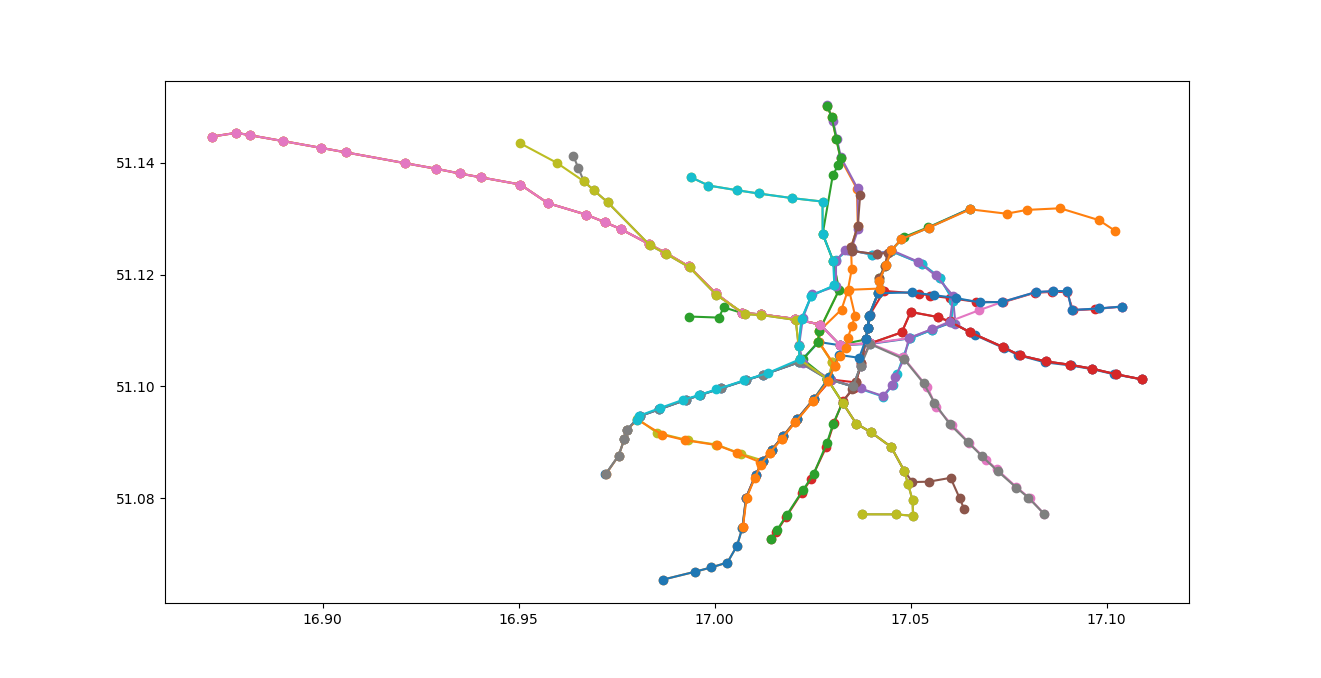
\includegraphics[width=1.0\textwidth]{images/graf.png}
	
	\caption{Graf ukazujący mape przystanków tramwajowych ułożony według współrzędnych}
	

	\end{figure}

\section{Wymagania}
Do działania programu wymagany jest Python 3 oraz biblioteki:
\begin{itemize}
    \item PyQt5 - biblioteka na licencji GPL odpowiadająca za GUI programu.
    \item matplotlib - biblioteka służąca do generowania wykresów.
\end{itemize}
Projekt zawiera plik \textit{requirements.txt}, za pomocą którego można zainstalować wszystkie potrzebne zależności.

\section{Algorytmy}

\subsection{Depth-first search}
Depth-first search, czyli przeszukiwanie w głąb. Algorytm startując z pewnego wierzchołka wrzuca na stos wszystkich jego sąsiadów. Następnie ściąga element ze stosu i powtarza operację. Algorytm może zostać zaimplementowany rekurencyjnie, jednak w tym przypadku nie zdecydowano się na to rozwiązanie. Dzięki zastosowaniu stosu, po zbadaniu wszystkich krawędzi wychodzących z danego wierzchołka algorytm powraca do wierzchołka, z którego dany wierzchołek został odwiedzony(ang. backtracing). Algorytm kończy swoje działanie w chwili znalezienia szukanego elementu.




	
\subsection {Breadth-first search} 
Przechodzenie grafu rozpoczyna się od zadanego wierzchołka i polega na odwiedzeniu wszystkich osiągalnych z niego wierzchołków. W praktyce implementacja BFS wygląda tak samo jak w przypadku DFS, różnicą jest zastosowanie kolejki zamiast stosu. Algorytm przeszukuje graf poziom po poziomie, w wyniku czego czas potrzebny na odszukanie drogi zazwyczaj jest dłuższy niż w przypadku DFS. Przeszukiwanie wszerz daje gwarancję odszukania drogi, w dodatku zawsze będzie ona najkrótsza względem przebytych wierzchołków, co daje przewagę temu algorytmowi nad przeszukiwaniem wgłąb. 



\subsection {A*}
Algorytm stosujący heurystykę w celu znalezienia najkrótszej ścieżki w grafie ważonym z dowolnego wierzchołka. Algorytm jest optymalny, w tym sensie, że znajduje ścieżkę, jeśli tylko taka istnieje, i przy tym jest to ścieżka najkrótsza. Algorytm, ze względu na heurystykę może być wykorzystany tylko jeśli graf jest zbudowany tak, żeby było możliwe oszacowanie realnej odległości między wierzchołkami. Mapa miasta spełnia ten warunek dzięki współrzędnym geograficznym w jakie wyposażony jest każdy przystanek (wierzchołek). Algorytm A* w odróżnieniu od innych algorytmów, dzięki heurystyce nie przeszukuje wierzchołków które oddalają go od celu. Do implementacji algorytmu zastosowano kolejkę priorytetową.

\section{Implementacja}
W poniższych podrozdziałach przedstawiono szczegóły implementacyjne wykonanego programu. 

\subsection{Graf}
Graf zaimplementowano metodą list sąsiedztwa (ang. \textit{adjacency list}). Zbudowany jest za pomocą słownika, który mapuje nazwy przystanków odpowiadającym im wierzchołkom grafu. Wierzchołek grafu jest zaimplementowany w osobnej strukturze, która zawiera informacje takie jak nazwa przystanku, listę sąsiedztwa, współrzędne geograficzne czy linie tramwajowe przejeżdżające przez dany przystanek.
\\
Każdy z algorytmów wyszukiwania zwracał znalezioną przez siebie ścieżkę oraz liczył ilość zakolejkowań oraz zdjęć z kolejki w celu statystyk. Na podstawie ścieżki ustalano przesiadki oraz weryfikowano optymalność.
\\
Dane do grafu pozyskane zostały z otwartych danych miasta Wrocław, następnie sparsowane przy użyciu biblitek xml.etree oraz csv języka Python.

\subsection{Realizacja przesiadek}
Po wyznaczeniu trasy należało poinformować użytkownika jakimi tramwajami może dostać się do celu. Zaprojektowano algorytm, który wykorzystuje fakt, że każdy z wierzchołków przechowuje informacje o liniach tramwajowych, które przez niego przejeżdżają. Dla każdego kolejnego przystanku w wyznaczonej trasie obliczano intersekcję (za pomocą funkcji STL - std::set\_intersection) linii z poprzednimi przystankami. Jeśli intersekcja okaże się zbiorem pustym, oznacza to przesiadkę na poprzednim przystanku. Operację powtarza się aż do końca trasy.

\subsection{Wizualizacja grafu}
Wszelkie wizualizacje dokonano za pomocą biblioteki matplotlib języka Python.

\subsection{GUI (Graphical User Interface)}
	\begin{figure}[H]
\centering

	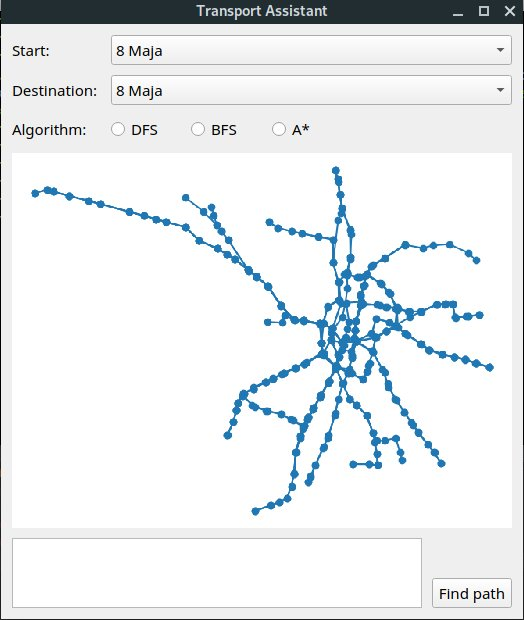
\includegraphics[width=0.5\textwidth]{images/gui.jpg}

\caption{GUI programu którego zadaniem jest wyszukanie linii tramwajowej przez 3 różne algorytmy przeszukiwania}
	\end{figure}
GUI programu zostało wykonane za pomocą języka Python i biblioteki PyQt5.
U góry okna programu są trzy opcje do wyboru. Pierwszą z nich jest przystanek początkowy, następną jest przystanek końcowy, a ostatnią jest wybór algorytmu przeszukiwania. Po odpowiednim ustawieniu tych opcji oraz nacisnięciu przycisku ,,Find path'' na oknie wyświetli się graf z zaznaczoną wybraną trasą, wymaganymi przesiadkami, listą wszystkich przystanków, oraz długością trasy.

\begin{figure}[ht]
\centering

	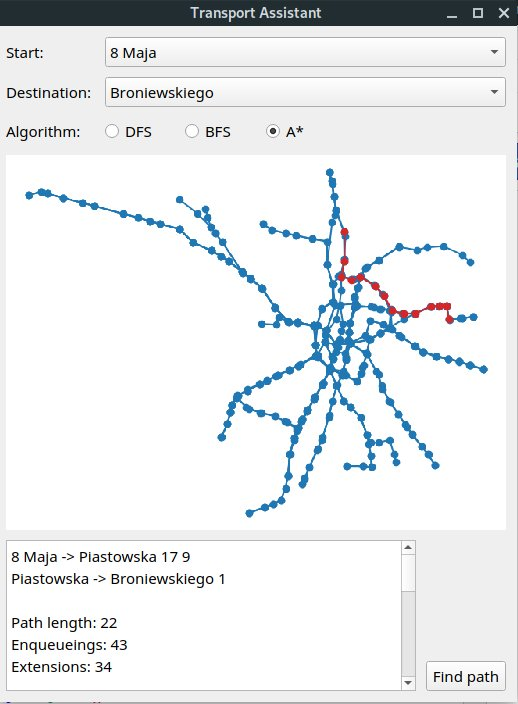
\includegraphics[width=0.5\textwidth]{images/find_example.jpg}

\caption{Przykładowe użycie programu.}
	\end{figure}

\section{Analiza}
W tym rozdziale zostały ukazane zaproponowane trasy opracowane przez każdy algorytm oraz porówanie czasów przeszukania grafu.

Na początku została wybrana trasa od przystanku ,,Klecina'' do przystanku ,,Dmowskiego''. Na obrazach poniżej zostały zaprezentowane poszczególne trasy zaproponowane przez poszczególne algorytmy.


\begin{figure}[ht]
	\centering
	\subfloat[Trasa zaproponowana przez DFS]{\label{odnosnik}
		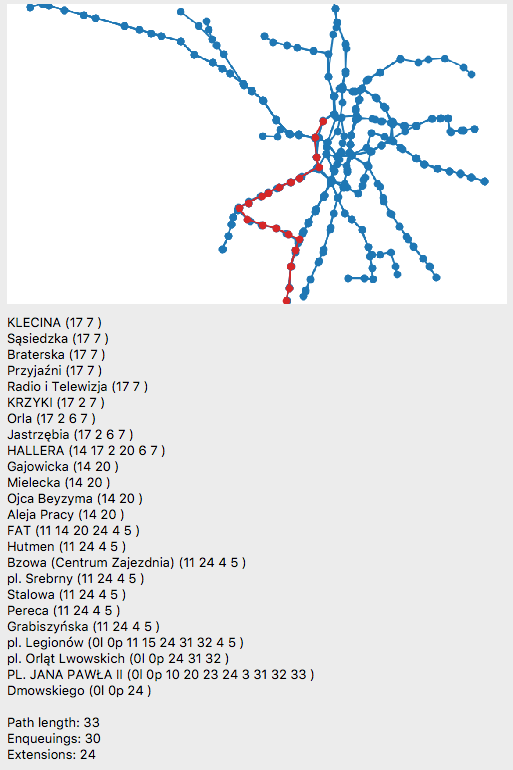
\includegraphics[width=0.3\textwidth]{images/klecina-dmowskiegoDFS.png}}
	\quad
	\subfloat[Trasa zaproponowana przez BFS]{\label{odnosnik}
		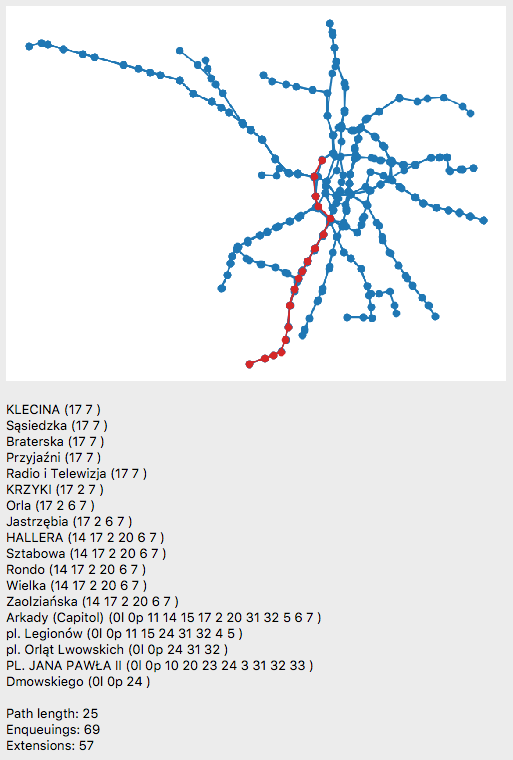
\includegraphics[width=0.3\textwidth]{images/klecina-dmowskiegoBFS.png}}
	\quad
	\subfloat[Trasa zaproponowana przez A*]{\label{odnosnik}
		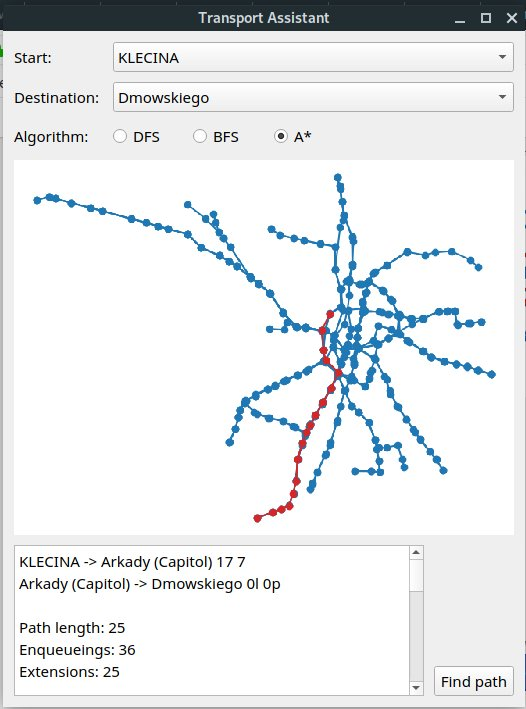
\includegraphics[width=0.3\textwidth]{images/klecina-dmowskiego-astar.jpg}}
	\quad
	\caption{Trasa z przystanku ,,Klecina'' do przystanku ,,Dmowskiego''}
\end{figure}	




Algorytm przeszukiwania w szerz oraz A* wybrały najbardziej optymalną trasę. Algorytm przeszukiwania wgłąb również wybrał dobrą trasę, ale waży ona więcej więc jest mniej optymalna niż trasa BFS i A*.

Najszybszy algorytm jeśli chodzi o wyznaczenie trasy był A*. Następnie był DFS, a na samym końcu BFS.

\newpage
Następną trasą jaka została wybrana była droga od przystanku ,,Leśnica'' do przystanku ,,Świdnicka''
\begin{figure}[ht]
	\centering

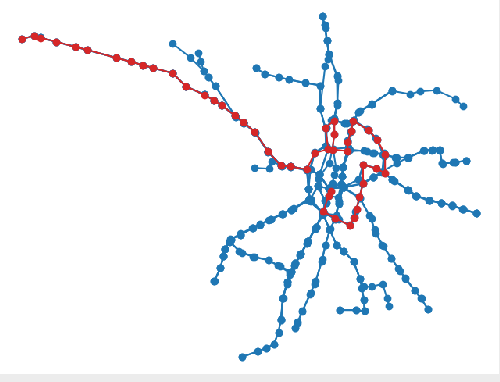
\includegraphics[width=0.5\textwidth]{images/mapa_lesnica-swidnicka.png}

\caption{Trasa z przystanku ,,Leśnica''-,,Świdnicka'' wyliczona za pomocą DFS.}
\end{figure}

\begin{figure}[H]
	\centering
	\subfloat[Trasa zaproponowana przez DFS]{\label{odnosnik}
		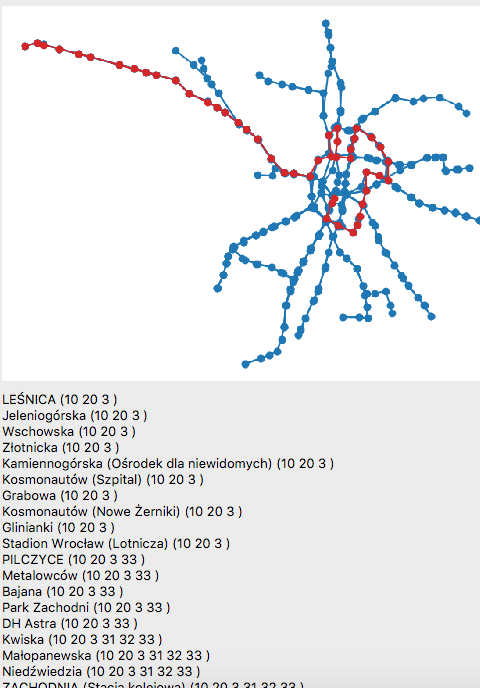
\includegraphics[width=0.3\textwidth]{images/lesnicka-swidnickaDFS.png}}
	\quad
	\subfloat[Trasa zaproponowana przez BFS]{\label{odnosnik}
		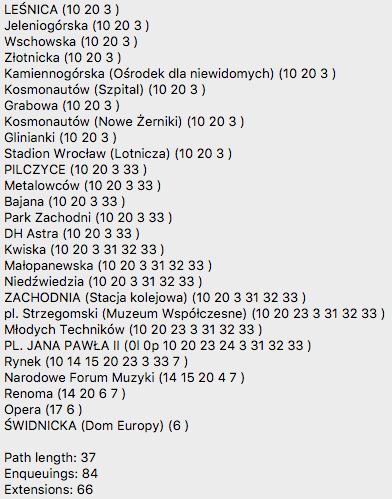
\includegraphics[width=0.3\textwidth]{images/lesnicka-swidnickaBFS.png}}
	\quad
	\subfloat[Trasa zaproponowana przez A*]{\label{odnosnik}
		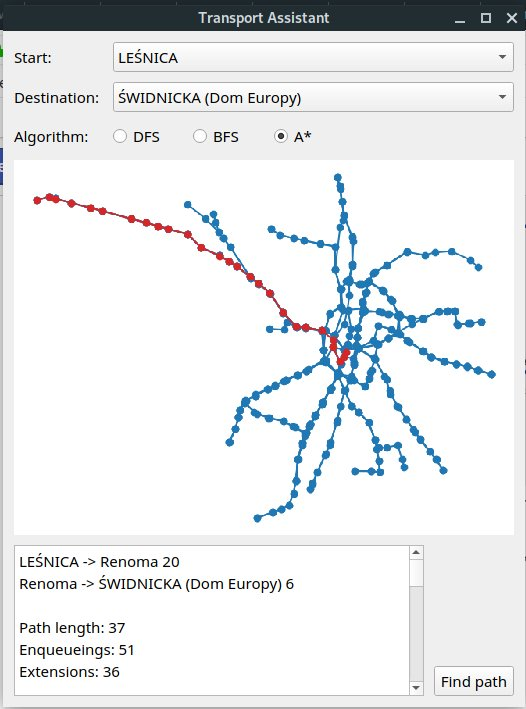
\includegraphics[width=0.3\textwidth]{images/lesnica-swidnicka-astar.jpg}}
	\quad
	\caption{Trasa z przystanku ,,Leśnica'' do przystanku ,,Świdnicka''}
\end{figure}	




\section {Wnioski}

Dla obu przypadków w poprzedniej sekcji można zauważyć:
\begin{itemize}
    \item Algorytm DFS szybko odnajduje swoją trasę, jednak nie jest ona ani optymalna ani nawet rozsądna.
    \item Algorytm BFS zawsze odnajduje rozsądną trasę, nawet optymalną, pod warunkiem, że wszystkie krawędzie grafu mają taką samą wagę.
    \item Algorytm A* w tym przypadku deklasuje pozostałe dwa algorytmy wyszukując zawsze optymalną trasę, rozwijając przy tym swoją ścieżkę do 5 razy rzadziej niż w przypadku BFS (dla trasy Leśnica-Stadion Olimpijski A* zanotował 37 rozszerzeń, BFS aż 156.). Niestety ze względu na heurystykę tego algorytmu nie można użyć w każdym przypadku.
\end{itemize}
\\
Nie zmierzono czasów działania poszczególnych algorytmów, ponieważ dysponowano zbyt małym zestawem danych, żeby czasy zauważalnie się różniły.
\\
Porównano obliczone trasy oraz wyznaczone przesiadki z trasami wyznaczonymi przez większe aplikacje tego typu (Google Maps, jakdojade), uzyskano wynik niemal identyczny, różniący się najprawdopodobniej w wyniku synchronizacji przesiadek.
\end{document}